\section{Game theory concepts}\label{sec:game_theory_intro}

In game theory there are several different forms of games.
This section outlines only the ones necessary for the formulation
of the scenario studied in this research project.
The first one is normal form games the second one is perfect information
extensive form games and the third one is extensive form games with imperfect
information.
The documentation of the python library \lstinline[style=pystyle]{nashpy} can
be used to find more information about the different types of games and concepts
that are discussed throughout this section.


\subsection{Normal form games}\label{sec:game_intro_normal_form_games}

Normal form games are strategic games that model strategic decision-makers.
These decision makers are referred to as players where each player has a
set of possible actions that they can take.
The game captures the interaction between the players by taking into account
the payoffs that each player receives for each possible combination of actions
taken by all players.
A strategic game consists of a set of players, a set of actions for each player,
and a payoff function that maps each combination of actions to a payoff for
each player~\cite{osborne2004_normal_form_games}.

Normal form games with \(2\) players are usually represented by \(2\)
matrices that include the payoffs for each player for every possible combination
of actions.
The set of available actions of a player is denoted by \(|S|\).
A pure strategy is a strategy that is associated with a single action \(i\) and
a mixed strategy \(\sigma\) is a strategy that is associated with a probability
distribution over the pure strategies \(\sigma_i\),
where \(\sum_i^{|S^k|}\sigma_i^k = 1\) for each player
\(k \in \{1,2,\dots n\}\).
A utility function \(u_k\) is a function that maps \(n\) strategy profiles (one
for each player) to a payoff for player \(k\).
The payoff for player \(k\) is given by \(u_k(\sigma^1, \sigma^2, \dots,
\sigma^n)\) where each \(\sigma^i\) represents a player. 

For example, consider the Prisoner's Dilemma game illustrated in
Table~\ref{tab:prisoners_dilemma}~cite{glynatsi2021bibliometric}.
In this game, player 1 can choose to either \textit{Cooperate} (C) or
\textit{Defect} (D) and player 2 can also choose to either \textit{Cooperate}
(C) or \textit{Defect} (D).

\begin{table}[H]
    \centering
    \caption{A game theoretic matrix representation of the Prisoner's Dilemma
    game}
    \begin{tabular}{|c|c|c|}
        \hline
        \backslashbox{Player 1}{Player 2} & Cooperate & Defect \\
        \hline
        Cooperate & \(3,3\) & \(0,5\) \\
        \hline
        Defect & \(5,0\) & \(1,1\) \\
        \hline
    \end{tabular}
    \label{tab:prisoners_dilemma}
\end{table}

An alternative way to represent the Prisoner's Dilemma game is by using the
payoff matrices in~\eqref{eq:prisoners_dilemma}.
The payoff matrix \(A\) shows the payoffs for player 1 and the payoff matrix
\(B\) shows the payoffs for player 2.
\begin{align}
    & \quad C \; D \nonumber \\
    A =
    \begin{pmatrix}
        3 & 0 \\
        5 & 1
    \end{pmatrix}
    \begin{matrix}
        C \\
        D
    \end{matrix} \qquad
    B =&
    \begin{pmatrix}
        3 & 5 \\
        0 & 1
    \end{pmatrix}
    \label{eq:prisoners_dilemma}
\end{align}

The entry in the first row and first column of both matrix \(A\) and matrix
\(B\) is \(3\).
That indicates that if both players choose to \textit{Cooperate} (i.e. player 1
chooses row 1 and player 2 chooses column 1) then they both receive a payoff of
\(u_1 = 3\) and \(u_2 = 3\).
Similarly, the entry in the second row and first column of matrix \(A\) is 0 and
the equivalent entry in matrix \(B\) is 5.
That indicates that if player 1 chooses to \textit{Defect} and player 2 chooses
to \textit{Cooperate} then player 1 receives a payoff of \(u_1 = 0\) and player
2 receives a payoff of \(u_2 = 5\).

Equivalently, a 3-player normal form game is represented by three 3-dimensional
matrices \(A\), \(B\) and \(C\).
The the rows of each matrix correspond to the actions of player 1, the columns
of each matrix correspond to the actions of player 2 and the third dimension of
each matrix corresponds to the actions of player 3.

\subsection{Nash Equilibrium}\label{sec:game_intro_nash_equilibrium}

The Nash equilibrium is a concept that was developed by John Nash in the
1950s.
It is a concept that is used to describe the behaviour of players in a
game when they are playing against each other~\cite{kreps1989nash}.
In essence, it is the state of the game where players are not able to improve
their payoff by changing their strategy.

\begin{definition}
In a 2-player game a player's strategy \(\hat{\sigma}^1\) is said to be a
\textbf{best response} to the opposing's player strategy \(\sigma^2\) if the
following holds:
\begin{equation}\label{eq:best_response}
    u_1(\hat{\sigma}^1,\sigma^2) \geq u_1(\sigma^1,\sigma^2) \quad
    \text{for all } \sigma^1 \in S^1
\end{equation}
\end{definition}

The Nash equilibrium is a pair of strategies for the two players where neither
player can improve their payoff by changing their strategy.
Thus the following definition can be built upon the best response definition.

\begin{definition}
A pair of strategies \(\hat{\sigma}^1\) and \(\hat{\sigma}^2\) is a Nash
equilibrium if they are both best responses to each other.
In other words, the following holds:
\begin{equation}\label{eq:nash_equilibrium}
    u_1(\hat{\sigma}^1,\sigma^2) \geq u_1(\sigma^1,\sigma^2)
    \quad \text{and} \quad
    u_2(\sigma^1, \hat{\sigma}^2) \geq u_2(\sigma^1,\sigma^2)
    \quad \text{for all } \sigma^1 \in S^1, \sigma^2 \in S^2
\end{equation}
\end{definition}

Consider the pig and piglet game where there are two players, the pig and the
piglet and two strategies each, to \textit{Push} (P) a lever or
\textit{Don't push} it (D).
The payoff matrices \(A\) and \(B\) for this game are shown
in~\eqref{eq:pig_piglet_payoff}.
\begin{align}
    & \quad P \; D \nonumber \\
    A =
    \begin{pmatrix}
        3 & 0 \\
        5 & 1
    \end{pmatrix}
    \begin{matrix}
        P \\
        D
    \end{matrix} \qquad
    B =&
    \begin{pmatrix}
        3 & 5 \\
        0 & 1
    \end{pmatrix}
    \label{eq:pig_piglet_payoff}
\end{align}

Consider the case where the pig is playing the \textit{Push} strategy.
The piglet's best response to the pig is to play the \textit{Don't push}
strategy as this will result in a higher payoff of \(u_2=3\) instead of
\(u_2=2\).
Similarly, if the pig is playing the \textit{Don't push} strategy then the
piglet's best response is still the \textit{Don't push} strategy as this will
result in a higher payoff of \(u_2=0\) instead of \(u_2=-1\).
Thus, regardless of the pig's strategy the piglet's best response is to play
the \textit{Don't push} strategy.
From the pig's perspective, if the piglet is playing the \textit{Don't push}
strategy then the pig's best response is to play the \textit{Push} strategy as
this will result in a higher payoff of \(2\) instead of \(0\).
Therefore, one possible pair of strategies that is a Nash equilibrium is
\(\sigma^1 = (1,0)\) and \(\sigma^2 = (0,1)\).
Note that \(\sigma = (p_1, p_2)\) where \(p_1\) is the probability of the player
playing the first strategy and \(p_2\) is the probability of the player
playing the second strategy. 

This in only an example of the Nash equilibrium where it only consisted of pure
strategies.
In general, the Nash equilibrium can consist of mixed strategies.
There are numerous algorithms that can be used to find the Nash equilibrium
of a game.
The algorithms that will be discussed in this section are the Lemke-Howson
algorithm and the support enumeration algorithm.


\subsubsection{Lemke-Howson Algorithm}

The Lemke-Howson algorithm is a method that can be used to find a Nash
equilibrium of a 2-player normal form game~\cite{LemkeHowson}.
Note that the algorithm is only applicable to 2-player normal form games and
the algorithm outputs only one Nash equilibrium.
The Lemke-Howson algorithm uses the concept of support enumeration described
in~\cite{nisan2007}
that is used to find all pairs of best responses for a given game.
For a non-degenerate 2-player game~\cite{degenerategames} the Lemke-Howson
algorithm performs the following steps:

\begin{enumerate}
    \item Obtain the best response polytopes \(P\) and \(Q\).
    \item Choose a starting label to drop, this will correspond to a vertex of
    \(P\) or \(Q\).
    \item In that polytope, remove the label from the corresponding vertex and
    move to the vertex that shared that label.
    A new label will be picked up and duplicated in the other polytope.
    \item In the other polytope drop the duplicate label and move to the vertex
    that shared that label.
\end{enumerate}
Repeat steps 3 and 4 until there are no duplicate labels.

The Lemke-Howson algorithm is implemented using the
\lstinline[style=pystyle]{nashpy} python library~\cite{thenashpyproject}.
The following code snippet shows how to use the Lemke-Howson algorithm to find
the Nash equilibrium of the pig and piglet game described in
equation~\eqref{eq:pig_piglet_payoff}.

\begin{lstlisting}[style=pystyle]
>>> import nashpy as nash
>>> import numpy as np
>>> A = np.array([[4, 2], [6, 0]])
>>> B = np.array([[2, 3], [-1, 0]])
>>> game = nash.Game(A, B)
>>> sigma_1, sigma_2 = game.lemke_howson(initial_dropped_label=0)
>>> sigma_1
array([1., 0.])
>>> sigma_2
array([0., 1.])

\end{lstlisting}

The outcome indicates that the Nash equilibrium of the pig and piglet game is
\(\sigma^1 = (1,0)\) and \(\sigma^2 = (0,1)\).
That is, the pig should always push the lever and the piglet should never push
the lever.
Consider the game of Rock-Paper-Scissors now where the payoff matrices are
shown in~\eqref{eq:rock_paper_scissors_payoff}.
\begin{align}
    & \quad \ R \quad \ P \quad \ S \nonumber \\
    A =
    \begin{pmatrix}
        0 & -1 & 1 \\
        1 & 0 & -1 \\
        -1 & 1 & 0
    \end{pmatrix}
    \begin{matrix}
        R \\
        P \\
        S
    \end{matrix} \qquad
    B = &
    \begin{pmatrix}
        0 & 1 & -1 \\
        -1 & 0 & 1 \\
        1 & -1 & 0
    \end{pmatrix}
    \label{eq:rock_paper_scissors_payoff}
\end{align}

By implementing the Lemke-Howson algorithm on the Rock-Paper-Scissors game, one
Nash equilibrium can be found.

\begin{lstlisting}[style=pystyle]
>>> A = np.array([
...     [1, -1, 0],
...     [0, 1, -1],
...     [-1, 0, 1]]
... )
>>> B = np.array([
...     [-1, 1, 0], 
...     [0, -1, 1],
...     [1, 0, -1]]
... )
>>> game = nash.Game(A, B)
>>> sigma_1, sigma_2 = game.lemke_howson(initial_dropped_label=0)
>>> sigma_1
array([0.33333333, 0.33333333, 0.33333333])
>>> sigma_2
array([0.33333333, 0.33333333, 0.33333333])

\end{lstlisting}

The outcome indicates that a Nash equilibrium of the Rock-Paper-Scissors game
is \(\sigma^1 = (1/3, 1/3, 1/3)\) and \(\sigma^2 = (1/3, 1/3, 1/3)\).
That is, the players should play each strategy with equal probability.


\subsubsection{Support Enumeration}

Another algorithm that can be used to find the Nash equilibrium of a 2-player
normal form game is the support enumeration algorithm.
The support enumeration algorithm can be used to find all Nash equilibria of a
non-degenerate 2-player normal form game~\cite{degenerategames} by using all
possible pairs of support of a game~\cite{myerson1997game}.
The following steps are performed by the support enumeration algorithm and
return all pairs of best responses in a game with payoff matrices \(A\) and
\(B\)~\cite{supportenumeration}:

\begin{enumerate}
    \item For all possible pairs of support \((M_x, N_y)\) of the mixed
    strategies \((x, y)\)
    \item Solve the following equations:
    \begin{align}
        \sum_{i \in M_x} x_i B_{ij} &= v, \quad \text{for all } j \in N_y \\
        \sum_{i \in M_x} x_i &= 1 \\
        \sum_{j \in N_y} y_j A_{ij} &= u, \quad \text{for all } i \in M_x \\
        \sum_{j \in N_y} y_j &= 1
    \end{align}
\end{enumerate}

The support enumeration algorithm is implemented using the
\lstinline[style=pystyle]{nashpy} python library~\cite{thenashpyproject}.
Consider the payoff matrices for the game of coordination shown
in~\eqref{eq:coordination_payoff}, where the two players would prefer to
perform the same action if possible, but player 1 has a slight preference
for action \(S_1\) and player 2 has a slight preference for action \(S_2\).
\begin{align}
    & \ \; S_1 \ S_2 \nonumber \\
    A =
    \begin{pmatrix}
        3 & 1 \\
        0 & 2
    \end{pmatrix}
    \begin{matrix}
        S_1 \\
        S_2
    \end{matrix} \qquad
    B = &
    \begin{pmatrix}
        2 & 1 \\
        0 & 3
    \end{pmatrix}
    \label{eq:coordination_payoff}
\end{align}

The following piece of code implements the support enumeration algorithm on the
coordination game and returns all Nash equilibria of the game.

\begin{lstlisting}[style=pystyle]
>>> A = np.array([
...     [3, 1],
...     [0, 2]
... ])
>>> B = np.array([
...     [2, 1],
...     [0, 3]
... ])
>>> game = nash.Game(A, B)
>>> nash1, nash2, nash3 = tuple(game.support_enumeration())
>>> nash1
(array([1., 0.]), array([1., 0.]))
>>> nash2
(array([0., 1.]), array([0., 1.]))
>>> nash3
(array([0.75, 0.25]), array([0.25, 0.75]))

\end{lstlisting}

The outcome indicates that there are three Nash equilibria of the coordination
game.
The first Nash equilibrium is \(\sigma^1 = (1, 0)\) and \(\sigma^2 = (1, 0)\),
which corresponds to both players playing action \(S_1\).
Similarly, the second Nash equilibrium is \(\sigma^1 = (0, 1)\) and
\(\sigma^2 = (0, 1)\), and corresponds to both players playing action \(S_2\).
The third Nash equilibrium is \(\sigma^1 = (\frac{3}{4}, \frac{1}{4})\) and
\(\sigma^2 = (\frac{1}{4}, \frac{3}{4})\), which means that player 1 should
play action \(S_1\) with probability \(\frac{3}{4}\) and action \(S_2\) with
probability \(\frac{1}{4}\) and player 2 should play action \(S_1\) with
probability \(\frac{1}{4}\) and action \(S_2\) with probability
\(\frac{3}{4}\).


\subsection{Learning Algorithms}\label{sec:game_intro_learning_algorithms}

Nash equilibria is a theoretical measure which can be inconsistent with
intuitive notions about what should be the outcome of a
game~\cite{myerson1978refinements}.
The concept of Nash equilibria is not always applicable to real-world
situations.
There are scenarios where a game has multiple Nash equilibria, but not all
of them can be reached by allowing the players to repeatedly play the game.
Evolutionary stable strategies (ESS) is a subsequent general concept that can
be more applicable to real-world situations~\cite{nowak1993evolutionary}.
Consider a population that consists of all possible strategies of a player and
stronger strategies can invade weaker ones strategies and replace them in this
population~\cite{smith1972game, smith1973logic}.
A strategy is an ESS if no other strategy can replace it or invade it from the
population of all strategies.
Note that all strategies that are ESS are also Nash equilibrium.
Learning algorithms can be used to reach certain ESS of a game.
The benefit of using learning algorithms and ESS, instead of calculating
the Nash equilibria, is that not only is it a more powerful concept of
equilibrium, but also the decision journey of the players can be observed.
Thus, players' decisions at each time step can be observed and the learning
process can be visualised.
There are numerous leaning algorithms that can be used to find ESS of a game.
In this subsection an overview of some of them will be given.

\subsubsection{Fictitious play}
One such learning algorithm is called Fictitious play~\cite{brownfictitiousplay,
fudenberg1998theory}.
The fictitious play algorithm is a sequential learning algorithm that is
based on the assumption that the players are rational and have perfect
information about the game.
At each time step, the players play a strategy that is based on the
previous actions of the opposing player.
In other words the players play a best response to their opponent's
empirical frequency of actions.

Once again, using the \lstinline[style=pystyle]{nashpy} python
library~\cite{thenashpyproject} the fictitious play algorithm can be
implemented on the following game.

\begin{lstlisting}[style=pystyle]
>>> A = np.array([
...     [4, 1, 3],
...     [2, 0, 2],
...     [3, 4, 1]
... ])
>>> B = np.array([
...     [4, 5, 1],
...     [2, 3, 2],
...     [6, 4, 0]
... ])
>>> game = nash.Game(A, B)
>>> np.random.seed(0)
>>> play_counts = list(game.fictitious_play(iterations=1000))
>>> play_counts[-1]
[array([642.,   0., 358.]), array([757., 243.,   0.])]

\end{lstlisting}

The output is the empirical frequency of actions played by each player.
The outcome indicates that the fictitious play algorithm converges to the
following Nash equilibrium: \(\sigma^1 = (\frac{2}{3}, 0, \frac{1}{3})\) and
\(\sigma^2 = (\frac{3}{4}, \frac{1}{4}, 0)\).
That is the outcome of the last iteration of the fictitious play algorithm and
normalised to sum to one.
Figure~\ref{fig:fictitious_play} shows all iterations of the fictitious play
algorithm and how the players converge to a Nash equilibrium.

\begin{figure}[H]
    \centering
    \includegraphics[width=0.45\textwidth]{chapters/04_game_theoretic_model/Bin/learning_algorithms_example/fictitious_row.pdf}
    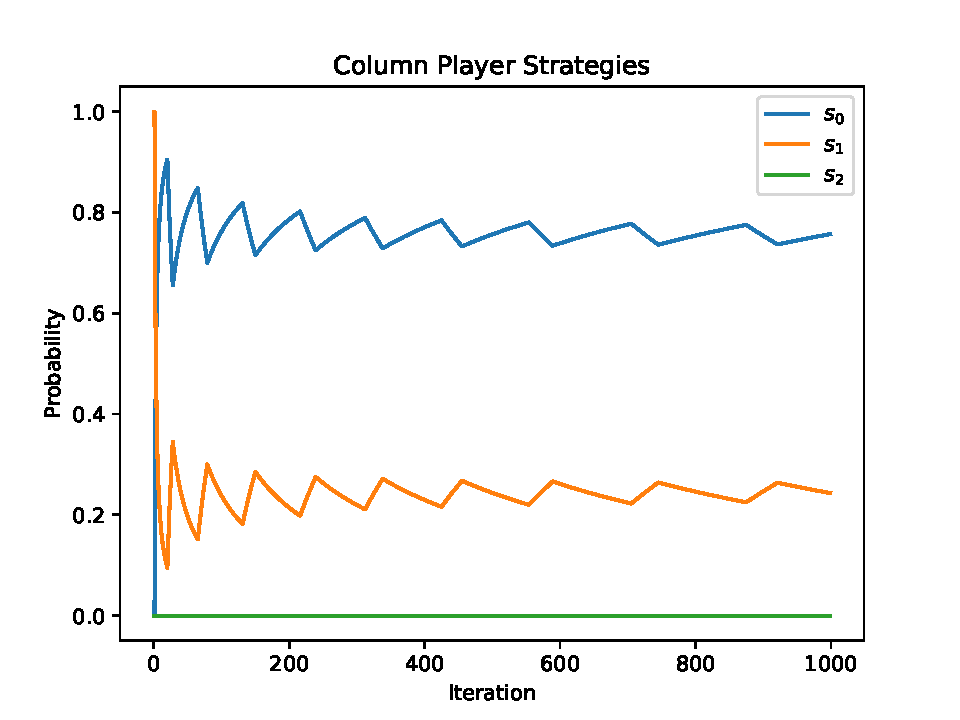
\includegraphics[width=0.45\textwidth]{chapters/04_game_theoretic_model/Bin/learning_algorithms_example/fictitious_col.pdf}
    \caption{Example of fictitious play algorithm run for \(1000\) iterations
    that converges to a Nash equilibrium.}
    \label{fig:fictitious_play}
\end{figure}


\subsubsection{Stochastic fictitious play}s
Another similar learning algorithm is called stochastic fictitious
play~\cite{hofbauerstochasticfictitous, fudenberg1998theory}.
Stochastic fictitious play is a variation of the fictitious play algorithm
where a stochastic perturbation \(\epsilon_i\) is added to each expected payoff
where \(\epsilon_i \in [0, \bar{\epsilon}]\) where \(\bar{\epsilon}\) is a
parameter needed for the algorithm.


\begin{lstlisting}[style=pystyle]
>>> A = np.array([
...     [4, 1, 3],
...     [2, 0, 2],
...     [3, 4, 1]
... ])
>>> B = np.array([
...     [4, 5, 1],
...     [2, 3, 2],
...     [6, 4, 0]
... ])
>>> game = nash.Game(A, B)
>>> np.random.seed(0)
>>> play_counts_and_distributions = tuple(
...     game.stochastic_fictitious_play(iterations=1000)
... )
>>> end_play_count, end_distribution = play_counts_and_distributions[-1]
>>> end_play_count
[array([624.,   0., 376.]), array([767., 233.,   0.])]

\end{lstlisting}

The output is the empirical probability of all actions played by player 1 and
player 2.
The outcome indicates that the stochastic fictitious play algorithm converges
to the following strategy: \(\sigma^1 = (\frac{2}{3}, 0, \frac{1}{3})\) and
\(\sigma^2 = (\frac{3}{4}, \frac{1}{4}, 0)\).
This is the outcome of the last iteration of the stochastic fictitious play
which is also similar to the fictitious play outcome.
Figure~\ref{fig:stochastic_fictitious_play} shows all iterations of the
stochastic fictitious play algorithm and how the players converge to a Nash
equilibrium.

\begin{figure}[H]
    \centering
    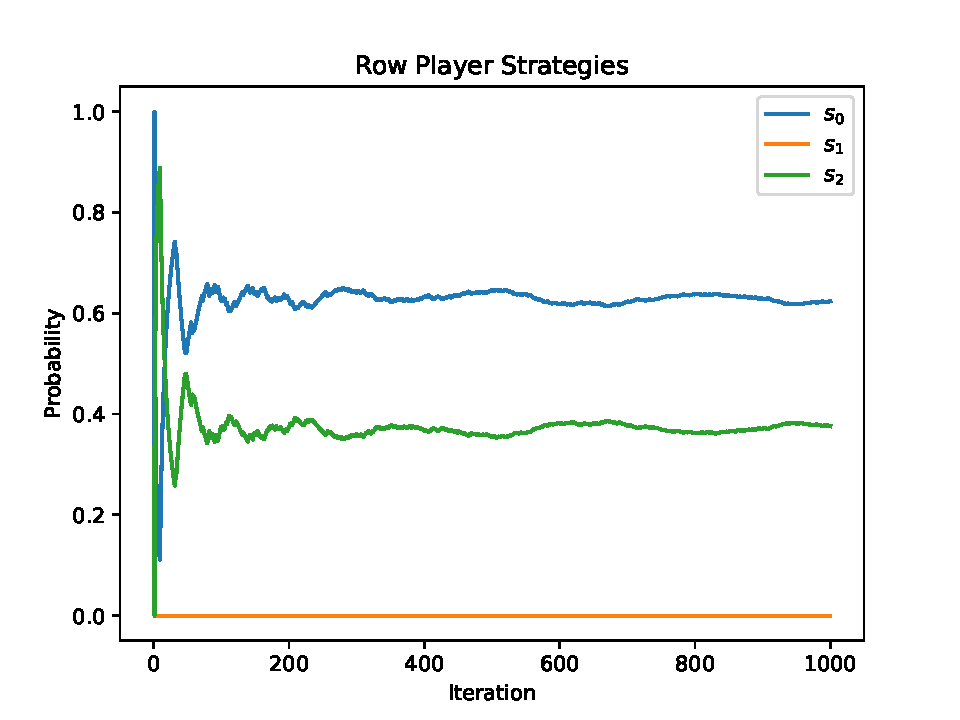
\includegraphics[width=0.45\textwidth]{chapters/04_game_theoretic_model/Bin/learning_algorithms_example/stochastic_row.pdf}
    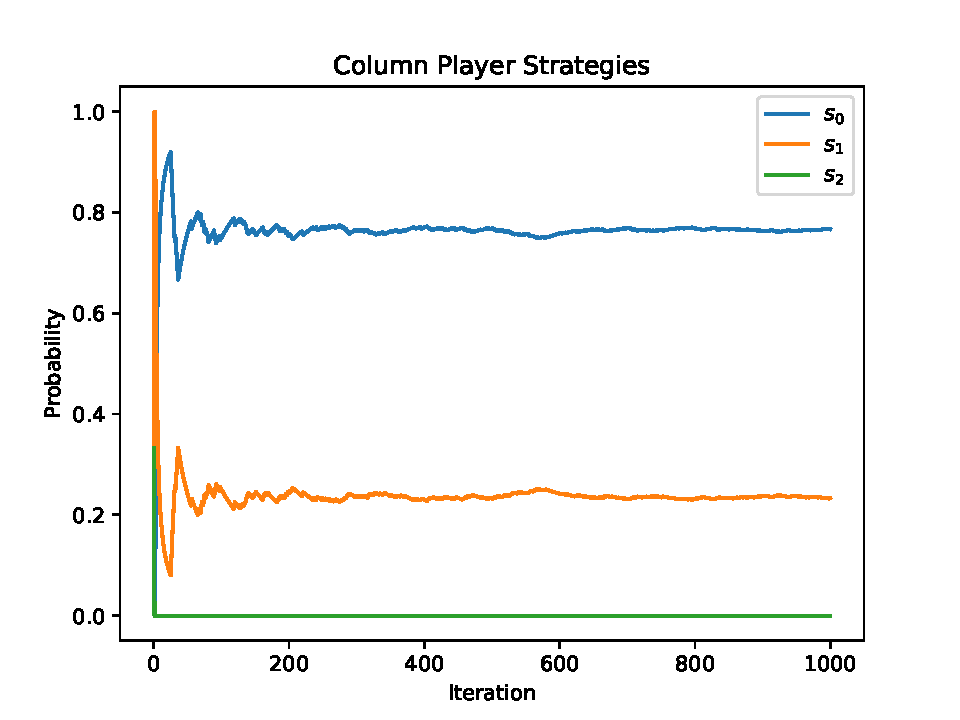
\includegraphics[width=0.45\textwidth]{chapters/04_game_theoretic_model/Bin/learning_algorithms_example/stochastic_col.pdf}
    \caption{Example of stochastic fictitious play algorithm for \(1000\)
    iterations that converges to a Nash equilibrium.}
    \label{fig:stochastic_fictitious_play}
\end{figure}


\subsubsection{Asymmetric replicator dynamics}

The learning algorithm that will be used most in this thesis is asymmetric
replicator dynamics~\cite{accinelli2011evolutionarily}.
Replicator dynamics is a learning algorithm that is used to express the
evolutionary dynamics of a population of players~\cite{komarova2004replicator}.
Consider a large population of some agents, also known as replicators.
Different types of such replicators meet and interact.
Each such interaction generates a certain payoff for each type of the
replicators.
This payoff is often referred to as the fitness of the replicator.
In evolutionary game theory these replicators are the strategies of the two
players.

Consider two types of individuals, \(A\) and \(B\), each with their own set of
strategies, \(S^A\) and \(S^B\).
Different strategies from \(S^A\) are assigned among the population of type
\(A\) and different strategies from \(S^B\) are assigned among the population
of type \(B\).
Individuals of type \(A\) are randomly paired with individuals of type \(B\)
and perform their assigned strategies.
As the game progresses the proportion of each strategy changes based on previous
interactions.
Given that the payoff matrices of the two players are \(A\) and \(B\), the
fitness of a strategy is given by:

\begin{equation}\label{eq:fitness_definition}
    f_x = A y \quad f_y = x^T B
\end{equation}

Note that \(x\) and \(y\) are the strategy vectors and correspond to the
population proportion of each strategy.
The average fitness of the two types of individuals is also given by:

\begin{equation}\label{eq:average_fitness_definition}
    \phi_x = f_x x^T \quad \phi_y = f_y y
\end{equation}

Finally the rate of change of the strategies are captured by the following
equations:

\begin{align}\label{eq:replicator_dynamics}
    \frac{dx}{dt} &= x_i((f_x)_i - \phi_x) \quad \text{for all } i \\
    \frac{dy}{dt} &= y_i((f_y)_i - \phi_y) \quad \text{for all } i
\end{align}

Asymmetric replicator dynamics is implemented by using the python
\lstinline[style=pystyle]{nashpy} library.
The following code snippet shows how to use the asymmetric replicator dynamics
algorithm to find the Nash equilibrium of a two-player game.
Consider the rock-paper-scissors game defined by the matrices
in~\eqref{eq:rock_paper_scissors_payoff}.

\begin{lstlisting}[style=pystyle]
>>> A = np.array([
...     [4, 1, 3],
...     [2, 0, 2],
...     [3, 4, 1]
... ])
>>> B = np.array([
...     [4, 5, 1],
...     [2, 3, 2],
...     [6, 4, 0]
... ])
>>> game = nash.Game(A, B)
>>> xs, ys = game.asymmetric_replicator_dynamics(
...     timepoints=np.linspace(0, 100, 100),
... )
>>> np.round(xs[-1], 4)
array([0.9207, 0.    , 0.0793])
>>> np.round(ys[-1], 4)
array([0.7429, 0.2571, 0.    ])

\end{lstlisting}

The output of the asymmetric replicator dynamics algorithm is the latest
population proportion of each strategy \(\sigma^1 = (0.92, 0, 0.08)\) and
\(\sigma^2 = (0.74, 0.25, 0)\).
That doesn't mean that the strategies have reached a steady state.
For this condition to be reached the rate of change of the strategies needs to
be \(\frac{dx}{dt} = \frac{dy}{dt} = 0\).
In fact Figure~\ref{fig:asymmetric_replicator_dynamics} shows that the
strategies played over time using the asymmetric replicator dynamics algorithm
have in fact not reached a steady state.

\begin{figure}[H]
    \centering
    \includegraphics[width=0.45\textwidth]{chapters/04_game_theoretic_model/Bin/learning_algorithms_example/asymmetric_rd_row.pdf}
    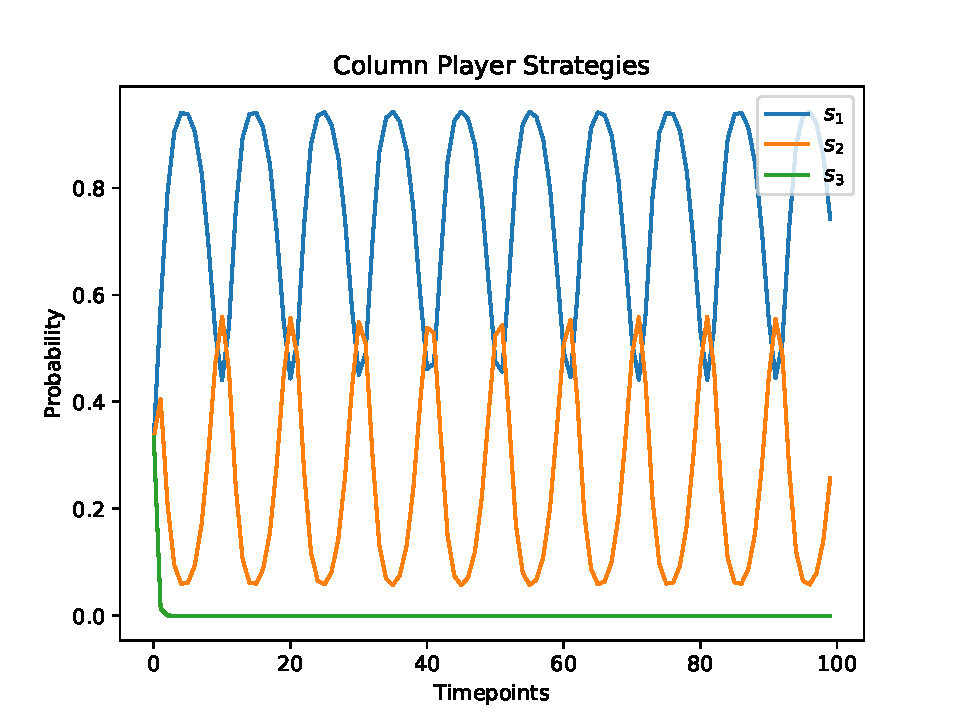
\includegraphics[width=0.45\textwidth]{chapters/04_game_theoretic_model/Bin/learning_algorithms_example/asymmetric_rd_col.pdf}
    \caption{Example of asymmetric replicator dynamics algorithm that does
    not converge.}
    \label{fig:asymmetric_replicator_dynamics}
\end{figure}

It can be seen that strategies player 1 alternates between strategy \(s_1\) and
\(s_3\) while player 2 alternates between strategy \(s_1\) and \(s_2\).
This game cannot reach a steady state given the uniform initial distribution of
the strategies.
Consider a different game where the steady strategy choice can be reached.

\begin{lstlisting}[style=pystyle]
>>> A = np.array([
...     [4, 1],
...     [2, 5],
... ])
>>> B = np.array([
...     [4, 5],
...     [2, 3],
... ])
>>> game = nash.Game(A, B)
>>> x0 = np.array([0.9, 0.1])
>>> y0 = np.array([0.9, 0.1])
>>> xs, ys = game.asymmetric_replicator_dynamics(
...     timepoints=np.linspace(0, 20, 100),
...     x0=x0,
...     y0=y0,
... )
>>> np.round(xs[-1], 4)
array([0., 1.])
>>> np.round(ys[-1], 4)
array([0., 1.])

\end{lstlisting}

The output of the asymmetric replicator dynamics algorithm is the latest
population proportion of each strategy \(\sigma^1 = (0, 1)\) and
\(\sigma^2 = (0, 1)\).
This indicates that the strategies have reached a steady state.
In replicator dynamics when a replicator is eliminated (in this case strategy
\(s_1\)), it cannot be recovered.
In addition, note that for this game the asymmetric replicator dynamics
algorithm was ran with a non-uniform initial distribution of the strategies.
In fact, even though the initial distribution of the strategies was
\(x_0 = (0.9, 0.1)\) and \(y_0 = (0.9, 0.1)\), strategy \(s_2\) still managed
to take over the population.

\begin{figure}[H]
    \centering
    \includegraphics[width=0.45\textwidth]{chapters/04_game_theoretic_model/Bin/learning_algorithms_example/asymmetric_rd_2_row.pdf}
    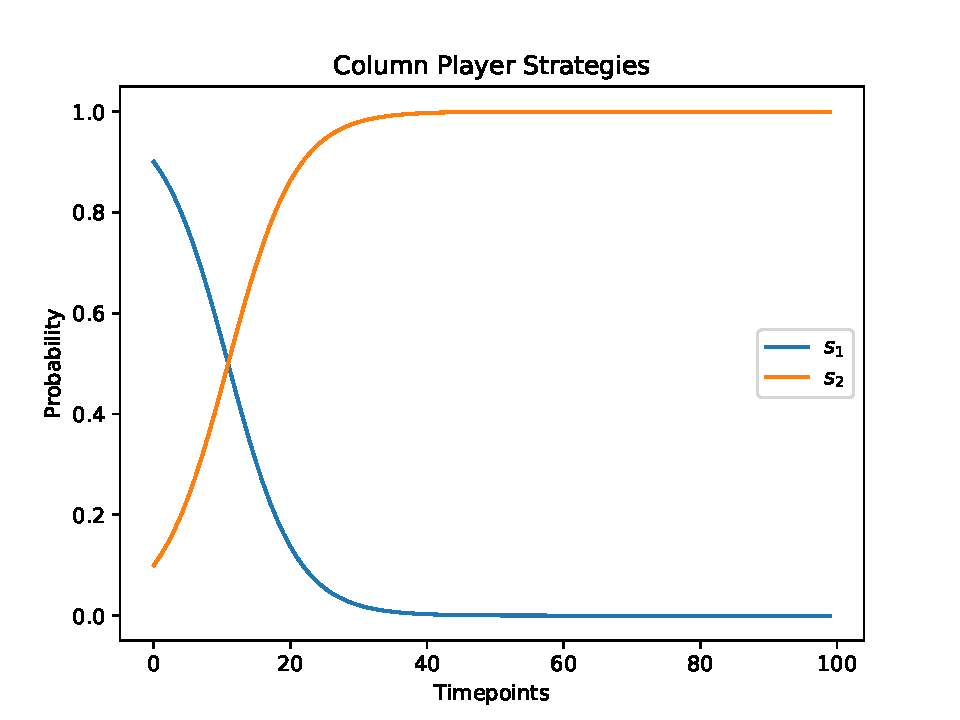
\includegraphics[width=0.45\textwidth]{chapters/04_game_theoretic_model/Bin/learning_algorithms_example/asymmetric_rd_2_col.pdf}
    \caption{Example of asymmetric replicator dynamics algorithm that converges}
    \label{fig:asymmetric_replicator_dynamics_steady}
\end{figure}


\subsection{Perfect-information extensive form game}

Unlike normal-form games extensive-form games work in a sequential way, where
players do not make decisions at the same time.
Instead, the first player chooses their strategy and then the opposing player,
fully aware of the choice made by the first player, chooses their own strategy.
There are numerous situations where decision makers can change their actions
based on the actions of other decision makers.
Such type of sequential games are also referred to as extensive form games.
One of the most common types of extensive form games is the perfect-information
extensive form game.
In this type of game, the players are assumed to have perfect information
about the previous actions of other
players.
There are four key components of a perfect-information extensive form game; the
players, the terminal nodes, the player function and the preferences of the
players~\cite{osborne2004_extensive_form_games}.
Examples of such games are the game of chess and the game of
Backgammon~\cite{hart1992games}.

Perfect information extensive form games are represented by a tree where the
nodes of the tree are the terminal nodes and represent the outcome of the
game.
The following figure shows an example of a perfect information extensive form
game.

\begin{figure}[H]
    \centering
    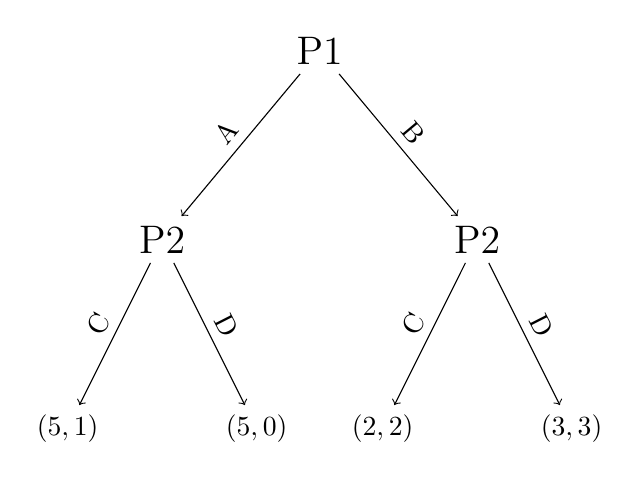
\begin{tikzpicture}[-, node distance = 2cm, scale=0.8]
    \node[anchor=north](P1){\Large{P1}};
    \node[anchor=north](P2_1) at (-2.5, -3) {\Large{P2}};
    \node[anchor=north](P2_2) at (2.5, -3) {\Large{P2}};

    \path[->] (P1) edge node [above, rotate=50] {A}(P2_1);
    \path[<-] (P2_2) edge node [above, rotate=310] {B}(P1);

    \node[anchor=north](F_1) at (-4, -6) {\((5,1)\)};
    \node[anchor=north](F_2) at (-1, -6) {\((5,0)\)};
    \node[anchor=north](F_3) at (1, -6) {\((2,2)\)};
    \node[anchor=north](F_4) at (4, -6) {\((3,3)\)};

    \path[->] (P2_1) edge node [above, rotate=60] {C}(F_1);
    \path[->] (P2_1) edge node [above, rotate=297] {D}(F_2);
    \path[->] (P2_2) edge node [above, rotate=60] {C}(F_3);
    \path[->] (P2_2) edge node [above, rotate=297] {D}(F_4);
\end{tikzpicture}

    \caption{Example of a perfect information extensive form game with \(2\)
    players and \(4\) terminal nodes.}
    \label{fig:extensive_form_game}
\end{figure}

Figure~\ref{fig:extensive_form_game} shows an example of a perfect information
extensive form game.
The game starts at the root node and the players take turns to make a move.
Player 1 can choose to either action A or action B.
Once player 1 has made a move, player 2 can choose to either action C or action
D, while having complete awareness of the action taken by player 1 and hence
their own position on the tree.
The final nodes of the tree represent the outcome of the game.
In this example, the outcome of the game is either 

\subsection{Imperfect-information extensive form game}
\label{sec:game_imperfect_information}

An imperfect information game is defined as an extensive form game where some
of the information about the game state is hidden for at least one of the
players~\cite{Berwanger2008}.
In other words, when making a decision, the players might not know their exact
position on the tree.
Similar to perfect information, imperfect information games are also represented
by a tree.
The following figure shows an example of an imperfect information extensive
form game.

\begin{figure}[H]
    \centering
    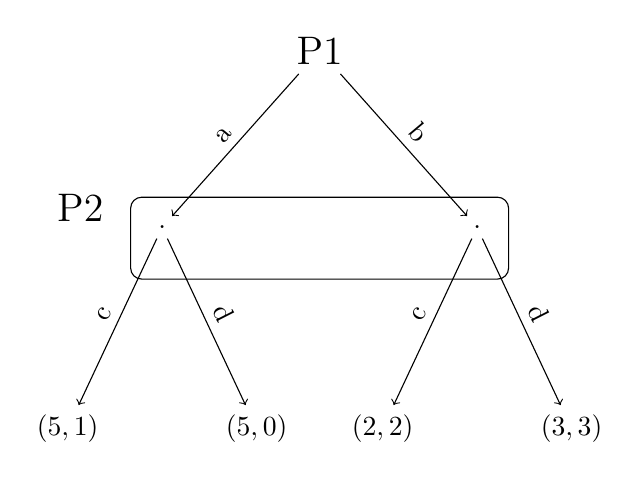
\begin{tikzpicture}[-, node distance = 2cm, scale=0.8]
    \node[anchor=north](P1){\Large{P1}};
    \node[anchor=north](P2_1) at (-2.5, -3) {.};
    \node[anchor=north](P2_2) at (2.5, -3) {.};
    \node[anchor=north](P2_3) at (-3.8, -2.5) {\Large{P2}};

    % \draw (0,-3.4) ellipse (3cm and 1cm);
    \draw[rounded corners] (-3, -4) rectangle (3, -2.7) {};

    \path[->] (P1) edge node [above, rotate=50] {a}(P2_1);
    \path[<-] (P2_2) edge node [above, rotate=310] {b}(P1);

    \node[anchor=north](F_1) at (-4, -6) {\((5,1)\)};
    \node[anchor=north](F_2) at (-1, -6) {\((5,0)\)};
    \node[anchor=north](F_3) at (1, -6) {\((2,2)\)};
    \node[anchor=north](F_4) at (4, -6) {\((3,3)\)};

    \path[->] (P2_1) edge node [above, rotate=60] {c}(F_1);
    \path[->] (P2_1) edge node [above, rotate=297] {d}(F_2);
    \path[->] (P2_2) edge node [above, rotate=60] {c}(F_3);
    \path[->] (P2_2) edge node [above, rotate=297] {d}(F_4);
\end{tikzpicture}

    \caption{An example of an imperfect information extensive form game with
    \(2\) players and \(4\) terminal nodes.}
    \label{fig:imperfect_extensive_form_game}
\end{figure}

Figure~\ref{fig:imperfect_extensive_form_game} shows an example of an imperfect
information extensive form game where player 2, when making their decision,
does not know whether they are in the left or right branch of the tree.
The game starts at the root node and the players take turns to make a move.
Player 1 can choose to either action \(a\) or action \(b\).
Once player 1 has made a move, player 2 can choose to either action \(c\) or
action \(d\), while having incomplete awareness of the action taken by player 1
and hence their own position on the tree.
The final nodes of the tree represent the outcome of the game.
This game can also be represented by a normal form game since both players end
up being completely unaware of the actions taken by the other player.
The payoff matrices in~\eqref{eq:imperfect_to_normal_form} show the normal form
game representation of the imperfect information extensive form game shown in
Figure~\ref{fig:imperfect_extensive_form_game}.
\begin{align}\label{eq:imperfect_to_normal_form}
    & \quad c \ \ d \nonumber \\
    A =
    \begin{matrix}
        a \\
        b
    \end{matrix}
    \begin{pmatrix}
        5 & 5 \\
        2 & 3
    \end{pmatrix} \quad
    B =&
    \begin{pmatrix}
        1 & 0 \\
        2 & 3
    \end{pmatrix}
\end{align}
